\section{Memristors Crossbar Array}\label{sec:crossbar}

Setting memristors in a crossbar array allows to perform analog \ac{VMM}, also called Multiply and Accumulate. This circuit works great for this use as all the computation is done almost instantly and using physics laws. \Cref{fig:crossbar} shows what a typical crossbar array looks like.

\begin{figure}[H]
  \centering
  \subfloat[Schematics, inspired from \cite{xbarFigures}]{\includesvg[width=.45\linewidth]{crossbar/crossbar}}%\qquad
  \hfill
  \subfloat[3 dimensional representation, from \cite{xbarFigures}]{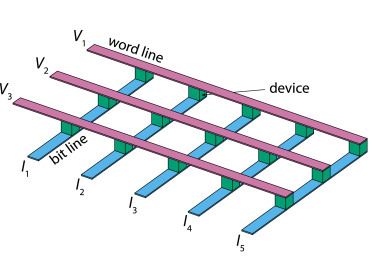
\includegraphics[width=.45\linewidth]{crossbar/crossbar3D.jpg}}\\
  \caption{Memristor crossbar array}
  \label{fig:crossbar}
\end{figure}

It uses physical properties of electrical systems to perform analog computing. In what follows I will use the circuit node in \cref{fig:crossNode} to explain the theory behind the memristor crossbar array.
\begin{figure}[H]
  \centering
  \includesvg[height=3.5cm]{crossbar/node}
  %\def\svgheigth{3.5cm}
  %\input{crossbar/node.pdf_tex}
  \caption{Memristor crossbar node of the $k^{th}$ line and $j^{th}$ column}
  \label{fig:crossNode}
\end{figure}

First of all, a voltage is applied on the $k^{th}$ line, because every column is virtually grounded, the voltage applied to the memristor, of a set resistance $\symR_k$, is $\symv_k$. As such and using Ohm's law, we know that the current flowing into the memristor ($\symi_{k}$) is bound by the following equation :

\begin{equation}
  \symv_k = \symR_k\cdot \symi_{k} \Rightarrow \symi_{k} = \symv_k\cdot (\frac{1}{\symR_k})= \symv_k\cdot \symG_k
\end{equation}
With $\symG_k$ being the conductance of memristor, defined as $\symG_k=\frac{1}{\symR_k}$.

This line then joins the column where a current of $\symi_{j,k-1}$ is flowing, then according to Kirchhoff's current law the resulting current is :
\begin{equation}
  \symi_{j,k} = \symi_{j,k-1}+\symi_{k} = \symi_{j,k-1} + \symv_k\cdot \symG_k
\end{equation}
By applying this process to the whole system we find that the current at the bottom of one column is :
\begin{equation}
  \symi_1= \symG_1\cdot \symv_1 +  \symG_2\cdot \symv_2 +  \symG_3\cdot \symv_3
\end{equation}
With $\symG_1$, $\symG_2$ and $\symG_3$ being the conductance of the 3 memristors in the first column.

Using such an analog circuit is a huge gain in time, for two main reasons :

\begin{itemize}
  \item By being analog, this circuit allows for analog computations which are much faster than their digital counterparts. As explained in this section, the circuit only uses physical properties of the different components and can compute large \acp{VMM} in a very short amount of time.
  \item The other advantage of such a system is the use of the memristors, that make the need to copy data from another memory useless as the memristors have a long term memory themselves. This is one of the ways to break down the Von Neumann bottleneck.
\end{itemize}
